\documentclass[a4paper,11pt]{article}


\usepackage[top=2cm, bottom=2cm, left=2cm, right=2cm]{geometry}
\setlength{\parskip}{10pt}

%% Mandatory stuff
\usepackage[utf8]{inputenc}
\usepackage[T1]{fontenc}

\usepackage{multicol}
%% Math package
\usepackage{amsmath}
\usepackage{amssymb}
\usepackage{amsfonts}
\usepackage{mathrsfs}
\DeclareMathAlphabet{\mathpzc}{OT1}{pzc}{m}{it}% Define a particular math font

%Advanced tabular managers
\usepackage{array}
\usepackage{multirow}

% Improve itemize environment
\usepackage{enumitem}
\setlist[itemize]{noitemsep, topsep=0pt}% Delete useless space

% In order to reduce the size after and before sections
\usepackage{titlesec}
\titlespacing*{\section}{0pt}{0.5pt}{0.5pt}

% Figure managers
\usepackage{graphicx}
\usepackage{float}

%\usepackage{subfig} %Like caption/subcaption but not compatible together.
\usepackage{caption}
\usepackage{subcaption}

%% Definition of a new environnement in order to make figure out of the margin
\newenvironment{changemargin}[2]{\begin{list}{}{%
\setlength{\topsep}{0pt}%
\setlength{\leftmargin}{0pt}%
\setlength{\rightmargin}{0pt}%
\setlength{\listparindent}{\parindent}%
\setlength{\itemindent}{\parindent}%
\setlength{\parsep}{0pt plus 1pt}%
\addtolength{\leftmargin}{#1}%
\addtolength{\rightmargin}{#2}%
}\item }{\end{list}}

%% Color package (for links, source code when using listings,...)
\usepackage[usenames]{color}
	%% Color for hyperlinks
\definecolor{colHyperlinks}{RGB}{0,90,170}%{59,0,159}

%
% Define pseudo-code environment and its layout
%
\usepackage{algorithm}
\usepackage{algpseudocode}

\errorcontextlines\maxdimen

% begin vertical rule patch for algorithmicx (http://tex.stackexchange.com/questions/144840/vertical-loop-block-lines-in-algorithmicx-with-noend-option)
\makeatletter
% start with some helper code
% This is the vertical rule that is inserted
\newcommand*{\algrule}[1][\algorithmicindent]{\makebox[#1][l]{\hspace*{.5em}\vrule height .75\baselineskip depth .25\baselineskip}}%

\newcount\ALG@printindent@tempcnta
\def\ALG@printindent{%
    \ifnum \theALG@nested>0% is there anything to print
        \ifx\ALG@text\ALG@x@notext% is this an end group without any text?
            % do nothing
            \addvspace{-3pt}% FUDGE for cases where no text is shown, to make the rules line up
        \else
            \unskip
            % draw a rule for each indent level
            \ALG@printindent@tempcnta=1
            \loop
                \algrule[\csname ALG@ind@\the\ALG@printindent@tempcnta\endcsname]%
                \advance \ALG@printindent@tempcnta 1
            \ifnum \ALG@printindent@tempcnta<\numexpr\theALG@nested+1\relax% can't do <=, so add one to RHS and use < instead
            \repeat
        \fi
    \fi
    }%
\usepackage{etoolbox}
% the following line injects our new indent handling code in place of the default spacing
\patchcmd{\ALG@doentity}{\noindent\hskip\ALG@tlm}{\ALG@printindent}{}{\errmessage{failed to patch}}
\makeatother
% end vertical rule patch for algorithmicx

% Set alignment of comments : now they are left aligned plus the comment symbol is now a triangle filled of black
\renewcommand{\algorithmiccomment}[1]{$\blacktriangleright$ #1}

% French translation of each keyword
\algrenewcommand\algorithmicend{\textbf{Fin}}
\algrenewcommand\algorithmicdo{\textbf{faire}}
\algrenewcommand\algorithmicwhile{\textbf{Tant que}}
\algrenewcommand\algorithmicfor{\textbf{Pour}}
\algrenewcommand\algorithmicforall{\textbf{Pour chaque}}
\algrenewcommand\algorithmicloop{\textbf{Boucler}}
\algrenewcommand\algorithmicrepeat{\textbf{Répéter}}
\algrenewcommand\algorithmicuntil{\textbf{Jusqu'à}}
\algrenewcommand\algorithmicprocedure{\textbf{Procédure}}
\algrenewcommand\algorithmicfunction{\textbf{Fonction}}
\algrenewcommand\algorithmicif{\textbf{Si}}
\algrenewcommand\algorithmicthen{\textbf{alors}}
\algrenewcommand\algorithmicelse{\textbf{Sinon}}
\algrenewcommand\algorithmicrequire{\textbf{Entrée:}}
\algrenewcommand\algorithmicensure{\textbf{Sortie:}}
\algrenewcommand\algorithmicreturn{\textbf{Retourner}}
\algrenewcommand\textproc{\textsc}
% Define new commands to begin and end an algorithm
\algnewcommand\algorithmicbegin{\textbf{Début}}
\algnewcommand\Begin{\item[\algorithmicbegin]}
\algnewcommand\algorithmicendbegin{\textbf{Fin}}
\algnewcommand\EndBegin{\item[\algorithmicendbegin]}

%% Hyperlinks for references (must be the last package loaded)
\usepackage[pdftex,%
  colorlinks,%
  linkcolor=colHyperlinks,%
  urlcolor=colHyperlinks,%
  citecolor=colHyperlinks,
  plainpages=false]{hyperref}
\begin{document}

\begin{center}
\Large{Licence L2\\Mathématiques pour l'informatique \\Partiel (1h30)}
\end{center}

\section*{Exercice 1}

Soit une relation d'ordre $\leq$ sur un ensemble $E$ définie par le diagramme de Hasse suivant :

\begin{figure}[h!]
	\centering
	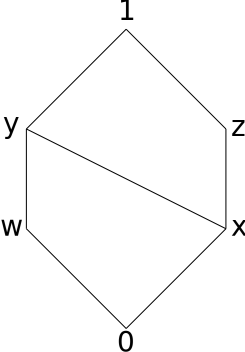
\includegraphics[width=0.15\linewidth]{./exo1.pdf}
\end{figure}

1) L'ensemble ordonné $(E, \leq)$ est-il un treillis? Justifiez votre réponse.

Correction : Un ensemble ordonné $(E, \leq)$ est un treillis si et seulement si $\forall a, b \in E $ il existe $a \wedge b$ et $a \vee b$.

Parmi les couples pouvant posés problèmes :

$z \vee y = 1$ et $z \wedge y = x$

$w \vee z = 1$ et $w \wedge z = 0$

$w \vee x = y$ et $w \wedge x = 0$

Les autres couples sont comparables et donc les bornes inférieur et supérieur sont respectivement le minimum et le maximum.

2) S'il s'agit d'un treillis, indiquer s'il est distributif, modulaire et/ou complémenté. Justifiez votre réponse.

Correction : premièrement, un treillis est distributif si on ne peut pas extraire ni de sous-treillis de type K ni de sous-treillis de type N. 

Dans notre cas, on ne peut extraire de sous-treillis de type type N, car, à partir de n'importe quel élément, il n'existe pas 3 autres éléments non comparable entre eux.

Ensuite, concernant les éventuelles sous-treillis de type K, on peut essayer avec les deux seules possibilités suivantes :
\begin{itemize}
	\item On tente de construire un sous-treillis $T_1$ en sélectionnant les éléments 0, w, z, y et 1. Ce n'est pas un sous-treillis car $y \wedge z = x \notin T_1$.
	\item On tente de construire un sous-treillis $T_2$ en sélectionnant les éléments 0, w, z, x et 1. Ce n'est pas un sous-treillis car $w \vee x = y \notin T_2$.
\end{itemize}

On ne peut donc pas construire de sous-treillis de type K non plus. Donc le treillis est distributif.

Deuxièmement, on sait qu'un treillis distributif est également modulaire. Puisque l'on vient de démontrer que le treillis est distributif, alors il est aussi modulaire.

Enfin, on souhaite montrer si le treillis est complémenté (c'est à dire que tout ses éléments possèdent un complément). Essayons de trouver le complément de $x$ :
\begin{itemize}
	\item $x \vee z = z \neq 1$. Donc $z$ n'est pas le complément de $x$.
	\item $x \vee w = y \neq 1$. Donc $x$ n'est pas le complément de $x$.
	\item $x \vee y = y \neq 1$. Donc $y$ n'est pas le complément de $x$.
\end{itemize}

Ainsi, $x$ ne possède pas de complément ce qui implique que le treillis n'est pas complémenté.

\section*{Exercice 2}

Soient deux graphes $G_1$ et $G_2$ définis par les représentations de la figure \ref{fig:graphs_exo4}.

\begin{figure}[!ht]
	\centering
	\subcaptionbox{$G_1$}[.25\linewidth][c]{
		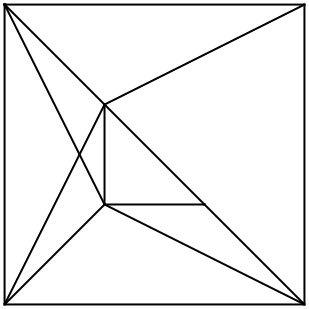
\includegraphics[width=.2\linewidth]{./graphe1.pdf}
	}
	\hspace{2cm}
	\subcaptionbox{$G_2$}[.25\linewidth][c]{
		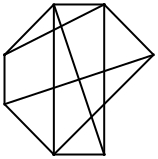
\includegraphics[width=.2\linewidth]{./graphe2.pdf}
	}
	\caption{}
	\label{fig:graphs_exo4}
\end{figure}

1) Parmi $G_1$ et $G_2$, indiquez celui qui est planaire et fournissez une représentation planaire lorsque cela est possible.

$G_1$ n'est pas un graphe planaire car on ne peut le représenter sans croiser au moins deux de ses arêtes.

$G_2$ est bien un graphe planaire car on peut le représenter tel que ci-dessous :

\begin{figure}[h!]
	\centering
	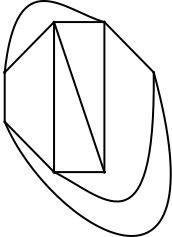
\includegraphics[width=0.25\linewidth]{./graphe2_correction.pdf}
\end{figure}

2) Pour le graphe planaire de la question précédente, indiquez son nombre de face, son nombre d'arêtes frontières et vérifier le théorème d'Euler.

Nombre de faces de $G_2$ : 7

Nombre d'arêtes frontières de $G_2$ : 12

Formule d'Euler : $f = m - n + c + 1$ tel que $f$ est le nombre de face, $m$ est le nombre d'arêtes, $n$ est le nombre de sommets et $c$ est le nombre de composantes connexes. Donc, pour $G_2$, $f = 12 - 7 + 1 + 1 = 7$.

3) Donnez la matrice d'adjacence du graphe non planaire.


\newpage
\begin{multicols}{2}
    Tout d'abords, on nomme les sommets du graphe comme sur la figure ci-dessous.

    \centering
    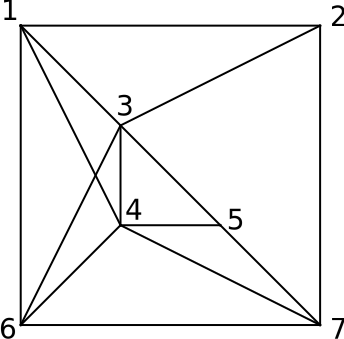
\includegraphics[width=0.2\textwidth]{./graphe1_correction.pdf}
    \captionof{figure}{$G_1$ avec ses sommets nommés}

    Ensuite, on construit $M_{G_1}$, la matrice d'adjacence du graphe $G_1$ tel que :
    $$M_{G_1} = 
    \bordermatrix{
        ~   & 1  & 2  & 3  & 4  & 5  & 6  & 7 \cr
        1   & 0  & 1  & 1  & 1  & 0  & 1  & 0 \cr
        2   & 1  & 0  & 1  & 0  & 0  & 0  & 1 \cr
        3   & 1  & 1  & 0  & 1  & 1  & 1  & 0 \cr
        4   & 1  & 0  & 1  & 0  & 1  & 1  & 1 \cr
        5   & 0  & 0  & 1  & 1  & 0  & 0  & 1 \cr
        6   & 1  & 0  & 1  & 1  & 0  & 0  & 1 \cr
        7   & 0  & 1  & 0  & 1  & 1  & 1  & 0 \cr
    }$$
\end{multicols}

\section*{Exercice 3}

L'algorithme de Kruskal (voir ci-dessous l'algorithme \ref{algo:kruskal}) a été proposé en 1956 par Joseph Kruskal. Il permet de rechercher un arbre couvrant de poids minimal à l'instar des algorithmes de Prim et de Sollin.

\begin{algorithm}
    \caption{Algorithme de Kruskal}
	\label{algo:kruskal}
    \begin{algorithmic}[1]
\Require 

	$G$ : le graphe à recouvrir

	$S$ : L'ensemble des sommets de $G$

	$A$ : l'ensemble des arêtes de $G$

\Ensure 

	$T$ : un arbre ou une forêt couvrant(e) de poids minimal du graphe G.

\Begin
	\State \Comment $T$ est l'arbre ou la forêt couvrant(e) à retourner
	\State \Comment à l'initialisation, $T$ contient autant de composante connexe que de sommets
    \State $T \leftarrow (S, \emptyset)$
    \State \Comment $A_t$ contient la liste des arêtes triés par ordre croissant de leur poids associé
    \State \Comment Ainsi, $A_t[0]$ correspond à l'arête de poids le plus faible
    \State \Comment et $A_t[\text{card}(S) - 1]$ correspond à l'arête de poids le plus fort
    \State $A_t \leftarrow$ trieCroissant($A$)
    \For{$i$ de $1$ à $\text{card}(S)-1$}
    	\State $a \leftarrow A_t[0]$
    	\State $A_t \leftarrow A_t \setminus a$
    	\If{$a$ connecte deux composantes connexes différentes}
    		\State $T \leftarrow T \cup a$
    	\EndIf
    \EndFor
    \State \Return $T$
\EndBegin
	\end{algorithmic}
\end{algorithm}

Soit le graphe $G_3$ défini par la représentation ci-dessous :
\begin{figure}[h!]
	\centering
	\includegraphics[width=0.25\linewidth]{./graphe3.pdf}
\end{figure}

1) Appliquer l'algorithme de Kruskal à $G_3$ en détaillant pour chaque itération $k$ : 
\begin{itemize}
	\item La liste des arêtes présentes dans $T_k$.
	\item Le poids $p(T_k)$ de $T_k$.
\end{itemize}

Correction :

Soit $G_3=(S,A)$.
Soient $T_k$ la forêt couvrante à l'itération $k$ et $P(T_k)$ le poids de l'arbre à l'itération K.

Initialisation :

$T = (S, \emptyset)$

$A_t = \{\{BE\}, \{BC\}, \{BA\}, \{DE\}, \{CF\}, \{DF\}, \{AE\}, \{EF\}\}$

$p(T_0) = 0$

Itération 1 :

$T_1 = (S, \{\{BE\}\})$

$P(T_1) = 1$

Itération 2 :

$T_2 = (S, \{\{BE\}, \{BC\}\})$

$P(T_2) = 3$

Itération 3 :

$T_3 = (S, \{\{BE\}, \{BC\}, \{BA\}\})$

$P(T_3) = 6$

Itération 4 :

$T_4 = (S, \{\{BE\}, \{BC\}, \{BA\}, \{DE\}\})$

$P(T_4) = 10$

Itération 5 :

$T_5 = (S, \{\{BE\}, \{BC\}, \{BA\}, \{DE\}, \{CF\}\})$

$P(T_5) = 15$

2) Représenter graphiquement l'arbre couvrant de poids minimal obtenu à la question 1).

\begin{figure}[h!]
	\centering
	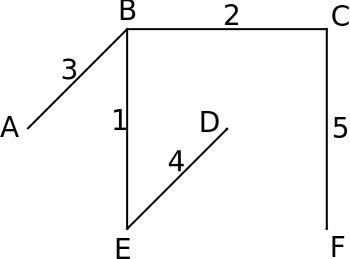
\includegraphics[width=0.25\linewidth]{./graphe3_correction.pdf}
\end{figure}

\section*{Exercice 4}

Après avoir spécifié la représentation informatique d'un graphe que vous allez utiliser, vous écrirez un algorithme qui retourne vrai si le graphe est connexe et faux sinon. Vous pourrez vous inspirez des algorithmes vu en cours.

Correction : On utilise la programmation orientée objet afin de représenter un graphe. La classe "Sommet" contient une variable "connexions" qui correspond à l'ensemble des sommets connectés au sommet courant par une arête. La classe "Graphe" possède la variable "sommets" correspondant à l'ensemble des sommets du graphe.

\begin{algorithm}
  \caption{estConnexe(G) de type booléen}
  \begin{algorithmic}[1]
\Require 

  $G$ : le graphe à tester

\Ensure 

  Vrai si $G$ est connexe, faux sinon.

\Begin
  \State \Comment{$M$ représente l'ensemble des sommets marqués}
  \State $M \leftarrow \emptyset$
  \State \Comment{$N$ représente l'ensemble des sommets non marqués}
  \State $N \leftarrow \text{G.sommets}$
  \State \Comment{$C$ représente l'ensemble des sommets à explorer}
  \State $C \leftarrow$ $\{$ un sommet quelconque de $N$ $\}$
  \While{$C \neq \emptyset$}
      \State $s_c \leftarrow C[0]$
      \State $M \leftarrow M \cup s_c$
      \State $N \leftarrow N \setminus s_c$
      \State $C \leftarrow C \setminus s_c$
      \ForAll{$s_v$ dans $s_c.\text{connexions}$}
          \If{$s_v \notin M$ et $s_v \notin C$}
              \State $C \leftarrow C \cup s_v$
          \EndIf
      \EndFor
  \EndWhile

  \If{$N \neq \emptyset$}
      \State \Comment{On n'a pas pu marquer tous les sommets}
      \State \Comment{donc le graphe n'est pas connexe}
      \State \Return faux
  \EndIf
  \State \Return vrai
\EndBegin
  \end{algorithmic}
\end{algorithm}

Il existe bien-sûr bien d'autre manière de mettre en évidence la connexité. Par exemple, l'algorithme de Prim s'arête s'il n'arrive pas à construire un arbre couvrant par manque de connexité...

\end{document}